% ─────────────────────────────────────────────────────────────────────────────
%  5343 Advanced Algorithms  |  Exam 02  |  Spring 2026  |  Version 3
%  80-minute condensed version with detachable answer sheet.
%
%  Toggle key:  uncomment \printanswers to produce the answer key.
%  Students write ONLY on the answer sheet (last two pages).
% ─────────────────────────────────────────────────────────────────────────────
\documentclass[12pt, addpoints]{exam}

\usepackage{amsmath, amssymb}
\usepackage[margin=0.75in, top=0.7in, bottom=0.7in]{geometry}
\usepackage{graphicx}
\usepackage{tikz}
\usetikzlibrary{positioning, arrows.meta, shapes.geometric}
\usepackage{array, booktabs}
\usepackage{multicol}
\usepackage{enumitem}
\usepackage{xcolor}
\usepackage{listings}
\usepackage{mdframed}
\usepackage{changepage}

% ── Answer-key toggle ────────────────────────────────────────────────────────
\printanswers

% ── Solution block ───────────────────────────────────────────────────────────
\definecolor{SolutionColor}{rgb}{0.93,0.96,0.93}
\newlength{\solindent}\setlength{\solindent}{0.5in}

\makeatletter
\renewenvironment{solution}[1][\unanswered]{%
  \def\@solvspace{#1}%
  \ifprintanswers
    \par\smallskip
    \begin{adjustwidth}{\solindent}{\solindent}
    \begin{mdframed}[backgroundcolor=SolutionColor, linewidth=0.4pt,
      linecolor=gray!60, innerleftmargin=5pt, innerrightmargin=5pt,
      innertopmargin=4pt, innerbottommargin=4pt, skipabove=0pt, skipbelow=0pt]%
  \else
    \setbox\z@\vbox\bgroup
  \fi
}{%
  \ifprintanswers
    \end{mdframed}%
    \end{adjustwidth}%
    \par\smallskip
  \else
    \egroup
    \ifdim\ht\z@>\z@\vspace{\ht\z@}\else\vspace{\@solvspace}\fi
  \fi
}
\makeatother

% ── Page style ───────────────────────────────────────────────────────────────
\pagestyle{headandfoot}
\firstpageheader{5343 Advanced Algorithms}{Exam 02 \textendash\ Spring 2026}%
  {\ifprintanswers\bfseries ANSWER KEY\else
   Page \thepage\ of \numpages\fi}
\runningheader{5343 Advanced Algorithms}{Exam 02}{Page \thepage\ of \numpages}
\firstpagefooter{}{\textit{Write all answers on the answer sheet. Do not write on this exam.}}{}
\runningfooter{}{\textit{Write all answers on the answer sheet.}}{}
\headrule\footrule

\pointsinmargin
\bracketedpoints

% ── Code style ───────────────────────────────────────────────────────────────
\lstset{basicstyle=\small\ttfamily, frame=single, language=Python,
        xleftmargin=1em, showstringspaces=false}

% ── Helpers ──────────────────────────────────────────────────────────────────
\newcommand{\blank}[1]{\underline{\hspace{#1}}}
\setlength{\columnsep}{1.4em}

% ── Ruled lines for answer sheet ─────────────────────────────────────────────
\newcommand{\answerlines}[1]{%
  \vspace{4pt}%
  \foreach \n in {1,...,#1}{%
    \noindent\rule{\linewidth}{0.3pt}\vspace{9pt}\newline}%
}

% ─────────────────────────────────────────────────────────────────────────────
\begin{document}

% ════════════════════════════════════════════════════════════════════════════
%  COVER
% ════════════════════════════════════════════════════════════════════════════
\begin{center}
  {\LARGE\bfseries 5343 Advanced Algorithms}\\[3pt]
  {\large Exam 02 \quad Spring 2026}
\end{center}

\smallskip
\noindent\textbf{Instructions:}
\begin{itemize}[nosep, leftmargin=*, topsep=2pt]
  \item Pencil only. Write all answers on the \textbf{detachable answer sheet} (last two pages).
  \item Use space wisely; align text for maximum readability.
  \item If you have a question, walk down and ask.
  \item Phones or other devices are grounds for failure.
\end{itemize}

\smallskip
\begin{center}
\renewcommand{\arraystretch}{1.35}
\begin{tabular}{|l|c|c|}
  \hline
  \textbf{Section} & \textbf{Points} & \textbf{Earned} \\\hline
  I. \ \ Multiple Choice (10 $\times$ 2) & 20 & \\\hline
  II. \ Fill in the Blank \ (5 $\times$ 2) & 10 & \\\hline
  III. Short Answer & 42 & \\\hline
  \textbf{Total} & \textbf{72} & \\\hline
\end{tabular}
\end{center}

\vspace{6pt}
\noindent\rule{\linewidth}{0.6pt}

% ════════════════════════════════════════════════════════════════════════════
\begin{questions}

% ════════════════════════════════════════════════════════════════════════════
\section*{Section I \quad Multiple Choice \hfill 2 pts each}
\addpoints
\noindent Circle the best answer on your answer sheet.
\vspace{4pt}

% \begin{multicols}{2}

\question[2]
Which container guarantees $O(1)$ access to the minimum element?
\begin{choices}
  \choice BST
  \choice Sorted Array
  \CorrectChoice Min-Heap
  \choice Hash Table
\end{choices}
\begin{solution}
  The heap property keeps the minimum at the root — O(1) access, O(log n) removal.
\end{solution}

\question[2]
Binary search requires which combination?
\begin{choices}
  \choice Sorted data only
  \choice O(1) index access only
  \CorrectChoice Sorted data \textbf{and} O(1) index access
  \choice A hash function and sorted data
\end{choices}
\begin{solution}
  Without O(1) index access, computing \texttt{mid} costs O(n) — no faster than linear.
\end{solution}

\question[2]
A hash table using linear probing has $\alpha = 0.90$.
Expected unsuccessful probes $\approx$:
\begin{choices}
  \choice 1.5
  \choice 2.5
  \choice 8.5
  \CorrectChoice 50.5
\end{choices}
\begin{solution}
  $\frac{1}{2}(1 + \frac{1}{(1-0.9)^2}) = \frac{1}{2}(101) = 50.5$.
\end{solution}

\question[2]
Heapify — building a min-heap from an unsorted array — runs in:
\begin{choices}
  \choice $O(\log n)$
  \choice $O(n \log n)$
  \CorrectChoice $O(n)$
  \choice $O(n^2)$
\end{choices}
\begin{solution}
  Most nodes are near the bottom and sift down few levels. The sum converges to O(n).
\end{solution}

\question[2]
Inorder traversal produces sorted output:
\begin{choices}
  \choice On any binary tree
  \CorrectChoice Only on a BST
  \choice Only on a complete binary tree
  \choice Only on a heap
\end{choices}
\begin{solution}
  Inorder exploits the BST ordering invariant. Without it, output order is arbitrary.
\end{solution}

\question[2]
A hash function $h(s) = \sum \texttt{ASCII}(s_i)$ violates:
\begin{choices}
  \choice Determinism
  \choice Uniformity
  \CorrectChoice Avalanche effect
  \choice Speed
\end{choices}
\begin{solution}
  ``abc'', ``bca'', and ``cab'' all produce the same sum.
  One changed character shifts the output by $\leq 1$ — far fewer than 50\% of bits.
\end{solution}

\question[2]
In a Huffman tree, the highest-frequency symbol gets:
\begin{choices}
  \CorrectChoice The shortest code — it sits closest to the root
  \choice The longest code — to distinguish it from others
  \choice A code equal in length to all other symbols
  \choice A code based on alphabetical order
\end{choices}
\begin{solution}
  Huffman always merges the two lowest-frequency nodes first, so high-frequency
  symbols stay near the root and accumulate fewer edge labels.
\end{solution}

\question[2]
Worst-case hash table lookup:
\begin{choices}
  \choice Chaining: O(1); open addressing: O(n)
  \choice Chaining: O(log n); open addressing: O(1)
  \choice Chaining: O(1); open addressing: O(log n)
  \CorrectChoice Both chaining and open addressing: O(n)
\end{choices}
\begin{solution}
  All n keys can hash to one slot (chaining: one chain of n;
  open addressing: one cluster of n). Expected O(1); worst-case O(n) for both.
\end{solution}

\question[2]
The MST of a connected graph is guaranteed unique when:
\begin{choices}
  \choice The graph is complete ($K_n$)
  \CorrectChoice All edge weights are distinct
  \choice The graph has no cycles
  \choice Both Prim's and Kruskal's agree on every edge
\end{choices}
\begin{solution}
  Distinct weights force the Cut Property to identify exactly one minimum crossing edge
  per cut — both algorithms are compelled to make the same choices.
\end{solution}

\question[2]
A symbol table is queried millions of times per second but updated once per minute.
Prefer:
\begin{choices}
  \choice Red-Black tree — fewer rotations means faster reads
  \CorrectChoice AVL tree — stricter balance means shorter tree and faster search
  \choice Either — they have identical search performance
  \choice Hash table — O(1) lookup regardless of update rate
\end{choices}
\begin{solution}
  AVL height $\leq 1.44\log n$ vs RB height $\leq 2\log n$.
  Fewer comparisons per lookup matters when reads dominate.
\end{solution}

% \end{multicols}

% ════════════════════════════════════════════════════════════════════════════
\vspace{4pt}
\noindent\rule{\linewidth}{0.4pt}
\section*{Section II \quad Fill in the Blank \hfill 2 pts each}
\addpoints
\noindent Write your answers on the answer sheet, numbered to match.
\vspace{4pt}

\question[2]
The load factor of a hash table is $\alpha =$ \blank{2in},
where $n$ = elements stored, $m$ = table capacity.
\begin{solution}$n/m$\end{solution}

\question[2]
Kruskal's algorithm uses \blank{2.6in} to detect whether adding an edge would form a cycle.
\begin{solution}Union-Find (Disjoint Set Union / DSU)\end{solution}

\question[2]
When inserting a node into a Red-Black tree, it is initially colored \blank{1.2in}.
\begin{solution}Red\end{solution}

\question[2]
A \blank{1.4in} tree compresses chains of single-child trie nodes into substring-labeled
edges, reducing node count from $O(\text{total chars})$ to $O(n)$ keys.
\begin{solution}Radix\end{solution}

\question[2]
In double hashing, $h_2(k)$ must never return \blank{0.6in}, or the probe sequence
revisits the same slot forever.
\begin{solution}0 (zero)\end{solution}

% ════════════════════════════════════════════════════════════════════════════
\vspace{4pt}
\noindent\rule{\linewidth}{0.4pt}
\section*{Section III \quad Short Answer}
\addpoints
\noindent\textit{Show your work. Write all answers on the answer sheet.}

% ── SA 1: Hash Table Trace (10 pts) ─────────────────────────────────────────
\question[10]
\textbf{Hash Table — Linear Probing.}
Table size $m = 11$, hash function $h(k) = k \bmod 11$.
Insert keys \textbf{22, 35, 15, 44, 55, 26} in order.

\begin{parts}
  \part[6] For each key, record $h(k)$, the probe sequence, and the final slot.
  Use the table on the answer sheet.

  \part[2] Draw the final table state on the answer sheet (slots 0–10; mark empty with \texttt{---}).

  \part[2] Name the clustering phenomenon visible in this trace and explain it in one sentence.
\end{parts}

\begin{solution}
  {\large \textbf{Solution}}\\

  \textbf{(a)}\\

  \begin{center}
  \renewcommand{\arraystretch}{1.3}
  \begin{tabular}{|c|c|l|c|}
    \hline Key & $h(k)$ & Probe sequence & Final slot\\\hline
    22 & 0 & 0 (empty) & 0 \\\hline
    35 & 2 & 2 (empty) & 2 \\\hline
    15 & 4 & 4 (empty) & 4 \\\hline
    44 & 0 & 0(22)$\to$1(empty) & 1 \\\hline
    55 & 0 & 0(22)$\to$1(44)$\to$2(35)$\to$3(empty) & 3 \\\hline
    26 & 4 & 4(15)$\to$5(empty) & 5 \\\hline
  \end{tabular}
\end{center}

  \textbf{(b)}\\
\begin{center}
    \begin{tabular}{|c|c|c|c|c|c|c|}
    \hline 0 & 1 & 2 & 3 & 4 & 5 & 6-7\\\hline
    22 &44 & 35 & 55 & 15 & 26 & --- \\\hline
  \end{tabular}
\end{center}
  \textbf{(c)}\\ 
  
  \textbf{Primary clustering}: keys hashing to different initial slots
  (0, 2, 4) pile into the same contiguous run (slots 0–5) because each collision
  extends the occupied block, forcing subsequent insertions to probe further.
\end{solution}

\newpage
% ── SA 2: AVL Rotations (12 pts) ────────────────────────────────────────────
\question[12]
\textbf{AVL Tree — Insertions and Rotations.}
Insert in order: $10,\ 20,\ 30,\ 15,\ 5,\ 25,\ 28$.

\noindent\textit{(a) After inserting 10, 20, 30 the tree is unbalanced.
  Name the imbalanced node, the rotation case, and draw the tree after the fix} \hfill (4 pts)


\begin{solution}

{\large \textbf{Solution}}\\

\begin{center}
\renewcommand{\arraystretch}{1.7}
No rotations until all values inserted. 
\begin{tabular}{|p{1.8in}|p{1.8in}|p{1.8in}|}
  \hline 
  10,20,30 Inserted & Balance Factors & Left Rotate at 20 \\\hline
  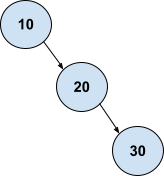
\includegraphics[width=100px]{./images/exam_2_avl_01.png} & 
  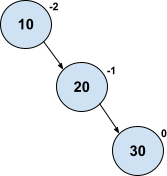
\includegraphics[width=100px]{./images/exam_2_avl_02.png} & 
  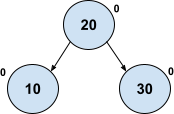
\includegraphics[width=100px]{./images/exam_2_avl_03.png} \\\hline
\end{tabular}
\end{center}
\end{solution}

\noindent\textit{(b) After inserting 15, 5, 25 — tree with balance factors} \hfill (4 pts)

\begin{solution}

\begin{center}
\renewcommand{\arraystretch}{1.7}
\begin{tabular}{|p{1.8in}|p{1.8in}|p{1.8in}|}
  \hline 
  Add 15 & Add 5 & Add 25 \\\hline
  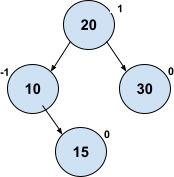
\includegraphics[height=100px]{./images/exam_2_avl_04_crop.png} & 
  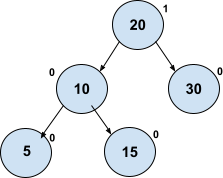
\includegraphics[height=100px]{./images/exam_2_avl_05_crop.png} & 
  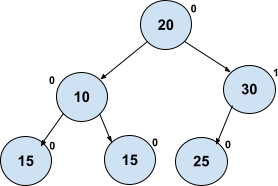
\includegraphics[height=100px]{./images/exam_2_avl_06_crop.png} \\\hline
\end{tabular}
\end{center}
\end{solution}

\noindent\textit{(c) After inserting 28 — rotation case, steps, final tree} \hfill (4 pts)

\begin{solution}

\begin{center}
\renewcommand{\arraystretch}{1.7}
\begin{tabular}{|p{1.8in}|p{1.8in}|p{1.8in}|}
  \hline 
  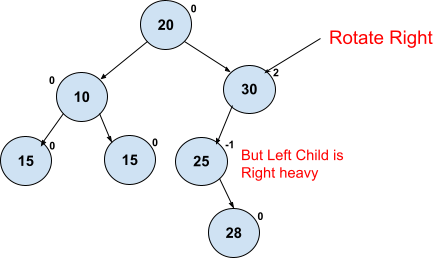
\includegraphics[height=100px]{./images/exam_2_avl_07_crop.png} & 
  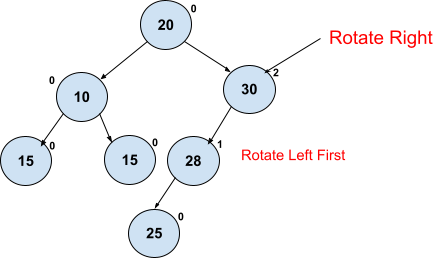
\includegraphics[height=100px]{./images/exam_2_avl_08_crop.png} & 
  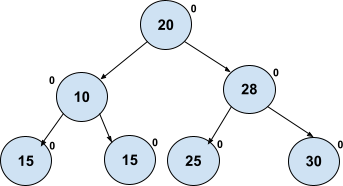
\includegraphics[height=100px]{./images/exam_2_avl_09_crop.png} \\\hline
\end{tabular}
\end{center}
\end{solution}

\newpage
% ── SA 3: Kruskal's (10 pts) ────────────────────────────────────────────────
\question[10]
\textbf{Minimum Spanning Tree — Kruskal's Algorithm.}

\begin{center}
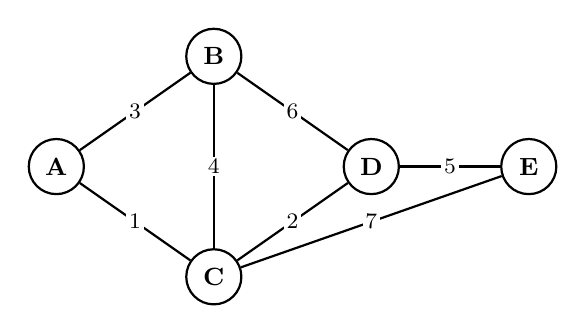
\begin{tikzpicture}[
    nd/.style={circle,draw,thick,minimum size=7mm,font=\small\bfseries},
    lbl/.style={font=\footnotesize,fill=white,inner sep=1pt}]
  \node[nd](A) at (0,1.8){A};
  \node[nd](B) at (2,3.2){B};
  \node[nd](C) at (2,0.4){C};
  \node[nd](D) at (4,1.8){D};
  \node[nd](E) at (6,1.8){E};
  \draw[thick](A)--node[lbl]{3}(B);
  \draw[thick](A)--node[lbl]{1}(C);
  \draw[thick](B)--node[lbl]{4}(C);
  \draw[thick](B)--node[lbl]{6}(D);
  \draw[thick](C)--node[lbl]{2}(D);
  \draw[thick](C)--node[lbl]{7}(E);
  \draw[thick](D)--node[lbl]{5}(E);
\end{tikzpicture}
\end{center}

\begin{parts}
  \part[6] Trace Kruskal's. Complete the table on the answer sheet (edges in sorted order,
  action, components after).

  \part[2] State the MST edges and total weight.

  \part[2] Why is the B--C edge skipped? Explain using Union-Find terminology.
\end{parts}

\begin{solution}

  {\large \textbf{Solution}}\\

  Sorted: A--C(1), C--D(2), A--B(3), B--C(4), D--E(5), B--D(6), C--E(7)

  \textbf{(a)}\\

  \begin{tabular}{|c|c|c|c|l|}\hline
  Step&Edge&Wt&Action&Components\\\hline
  1&A--C&1&Add&\{A,C\}\{B\}\{D\}\{E\}\\\hline
  2&C--D&2&Add&\{A,C,D\}\{B\}\{E\}\\\hline
  3&A--B&3&Add&\{A,B,C,D\}\{E\}\\\hline
  4&B--C&4&Skip&\{A,B,C,D\}\{E\}\\\hline
  5&D--E&5&Add&\{A,B,C,D,E\}\\\hline
  6&B--D&6&Skip&\{A,B,C,D,E\}\\\hline
  7&C--E&7&Skip&\{A,B,C,D,E\}\\\hline
  \end{tabular}

    \textbf{(b)}\\

  MST: A--C(1), C--D(2), A--B(3), D--E(5). Weight = \textbf{11}.\\

  \textbf{(c)}\\

  \texttt{find(B)==find(C)} — both in \{A,B,C,D\}. Adding the edge would close a cycle.

\end{solution}

\newpage
% ── SA 4: Huffman (10 pts) ──────────────────────────────────────────────────
\question[10]
\textbf{Huffman Tree — Build and Encode.}

\begin{center}
\renewcommand{\arraystretch}{1.2}
\begin{tabular}{|c|c||c|c|}
  \hline
  \textbf{Char} & \textbf{Freq} & \textbf{Char} & \textbf{Freq}\\\hline
  A & 12 & D & 4 \\\hline
  B &  7 & E & 3 \\\hline
  C &  5 & F & 2 \\\hline
\end{tabular}
\quad Total: 33
\end{center}

\begin{parts}
  \part[3] Trace the 5 min-heap merge steps on the answer sheet
  (left node, right node, new weight).

  \part[3] Draw the resulting tree on the answer sheet
  (0 = left edge, 1 = right edge).

  \part[4] Complete the encoding table on the answer sheet and compute:
  total Huffman bits, total fixed 3-bit bits, and bits saved.
\end{parts}

\begin{solution}
  {\large \textbf{Solution}}\\

  \textbf{(a)}\\

  Initial: F(2), E(3), D(4), C(5), B(7), A(12)\\

\begin{center}
\renewcommand{\arraystretch}{1.7}
\begin{tabular}{|c|c|c|c|{2.5in}|}
  \hline
  \textbf{Step} & \textbf{Left Weight} & \textbf{Right Weight} & \textbf{New Weight} \\\hline
  1 & F(2) & E(3) & 5 \\\hline
  2 & D(4)& C(5)&9 \\\hline
  3 & FE(5)& B(7)& 12 \\\hline
  4 & CD(9)&A(12) &21 \\\hline
  5 & FEB(12)& ACD(21)& 33\\\hline
\end{tabular}
\end{center}

  \textbf{(b)}\\
  
  Root(33): left FEB(12), right DCA(21).\\
  FEB: left FE(5)→left F(2)/right E(3); right B(7).\\
  DCA: left DC(9)→left D(4)/right C(5); right A(12).\\

  \textbf{(c)}\\
  
  \begin{tabular}{|c|c|c|c|c|}\hline
  Char&Freq&Code&Len&Bits\\\hline
  A&12&11&2&24\\\hline B&7&01&2&14\\\hline
  C&5&101&3&15\\\hline D&4&100&3&12\\\hline
  E&3&001&3&9\\\hline F&2&000&3&6\\\hline
  \multicolumn{4}{|r|}{Huffman total:}&80\\\hline
  \multicolumn{4}{|r|}{Fixed 3-bit ($33\times3$):}&99\\\hline
  \multicolumn{4}{|r|}{Saved:}&19\\\hline
  \end{tabular}
\end{solution}

\end{questions}

% ════════════════════════════════════════════════════════════════════════════
%  ANSWER SHEET  (detach and submit — keep exam booklet at your seat)
% ════════════════════════════════════════════════════════════════════════════
\newpage
\thispagestyle{empty}

\begin{center}
  {\LARGE\bfseries Answer Sheet --- Exam 02}\\[4pt]
  {\large 5343 Advanced Algorithms \quad Spring 2026}
\end{center}

\noindent
\begin{tabular}{@{}lll@{}}
  Name: & \makebox[2.6in]{\hrulefill} &
  Total: \makebox[0.6in]{\hrulefill} / 72 \\
\end{tabular}

\vspace{8pt}
\noindent\rule{\linewidth}{0.6pt}

\newpage
% ── I. Multiple Choice ───────────────────────────────────────────────────────
\noindent\textbf{Section I \ — \ Multiple Choice} \hfill \textit{2 pts each \ / 20 total}

\vspace{6pt}
\begin{center}
\renewcommand{\arraystretch}{1.6}
\begin{tabular}{|c|>{\centering\arraybackslash}p{0.55in}|>{\centering\arraybackslash}p{0.55in}|>{\centering\arraybackslash}p{0.55in}|>{\centering\arraybackslash}p{0.55in}|c|}
  \hline
  \textbf{Q} & \textbf{A} & \textbf{B} & \textbf{C} & \textbf{D} & \textbf{Pts} \\\hline
  1  & & & & & \hspace{0.4in} \\\hline
  2  & & & & & \\\hline
  3  & & & & & \\\hline
  4  & & & & & \\\hline
  5  & & & & & \\\hline
  6  & & & & & \\\hline
  7  & & & & & \\\hline
  8  & & & & & \\\hline
  9  & & & & & \\\hline
  10 & & & & & \\\hline
\end{tabular}
\end{center}

\vspace{6pt}
\noindent\rule{\linewidth}{0.4pt}

% ── II. Fill in the Blank ───────────────────────────────────────────────────
\noindent\textbf{Section II \ — \ Fill in the Blank} \hfill \textit{2 pts each \ / 10 total}

\vspace{4pt}
\renewcommand{\arraystretch}{2.0}
\begin{tabular}{@{}>{\bfseries}r p{5.0in} r@{}}
  1. & \hrulefill & \hspace{0.3in}/2 \\
  2. & \hrulefill & /2 \\
  3. & \hrulefill & /2 \\
  4. & \hrulefill & /2 \\
  5. & \hrulefill & /2 \\
\end{tabular}

\vspace{6pt}
\noindent\rule{\linewidth}{0.4pt}
\newpage
% ── III. Short Answer — SA1 & SA2 headers ───────────────────────────────────
\noindent\textbf{Section III \ — \ Short Answer} \hfill \textit{/42 total}

\bigskip
\noindent\textbf{SA1 — Hash Table Trace} \hfill \textit{/10}

\vspace{4pt}
\noindent\textit{(a) Probe trace \hfill (6 pts)}

\noindent\textit{(b) Final table state \hfill (2 pts)}

\noindent\textit{(c) Clustering phenomenon \hfill (2 pts)}

\begin{solution}
  \textbf{(a)}
  \renewcommand{\arraystretch}{1.3}
  \begin{tabular}{|c|c|l|c|}
    \hline Key & $h(k)$ & Probe sequence & Final slot\\\hline
    22 & 0 & 0 (empty) & 0 \\\hline
    35 & 2 & 2 (empty) & 2 \\\hline
    15 & 4 & 4 (empty) & 4 \\\hline
    44 & 0 & 0(22)$\to$1(empty) & 1 \\\hline
    55 & 0 & 0(22)$\to$1(44)$\to$2(35)$\to$3(empty) & 3 \\\hline
    26 & 4 & 4(15)$\to$5(empty) & 5 \\\hline
  \end{tabular}

  \textbf{(b)} Slot 0:22, 1:44, 2:35, 3:55, 4:15, 5:26, 6–10: ---

    \begin{tabular}{|c|c|c|c|c|c|c|}
    \hline 0 & 1 & 2 & 3 & 4 & 5 & 6-7\\\hline
    22 &44 & 35 & 55 & 15 & 26 & --- \\\hline
  \end{tabular}


  \textbf{(c)} \textbf{Primary clustering}: keys hashing to different initial slots
  (0, 2, 4) pile into the same contiguous run (slots 0–5) because each collision
  extends the occupied block, forcing subsequent insertions to probe further.
\end{solution}

\noindent\rule{\linewidth}{0.4pt}

\newpage
% ── SA2 ─────────────────────────────────────────────────────────────────────
\noindent\textbf{SA2 — AVL Rotations} \hfill \textit{/12}

\vspace{2pt}
\noindent\textit{(a) After inserting 10, 20, 30 — rotation case and result tree} \hfill (4 pts)

\begin{solution}

\begin{center}
\renewcommand{\arraystretch}{1.7}
No rotations until all values inserted. 
\begin{tabular}{|p{1.8in}|p{1.8in}|p{1.8in}|}
  \hline 
  10,20,30 Inserted & Balance Factors & Left Rotate at 20 \\\hline
  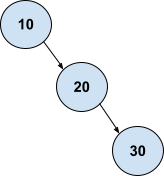
\includegraphics[width=100px]{./images/exam_2_avl_01.png} & 
  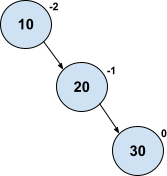
\includegraphics[width=100px]{./images/exam_2_avl_02.png} & 
  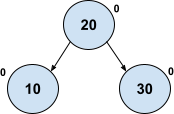
\includegraphics[width=100px]{./images/exam_2_avl_03.png} \\\hline
\end{tabular}
\end{center}
\end{solution}

\noindent\textit{(b) After inserting 15, 5, 25 — tree with balance factors} \hfill (4 pts)

\begin{solution}

\begin{center}
\renewcommand{\arraystretch}{1.7}
\begin{tabular}{|p{1.8in}|p{1.8in}|p{1.8in}|}
  \hline 
  Add 15 & Add 5 & Add 25 \\\hline
  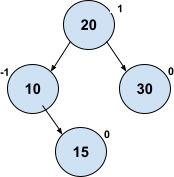
\includegraphics[height=100px]{./images/exam_2_avl_04_crop.png} & 
  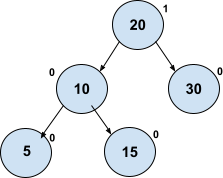
\includegraphics[height=100px]{./images/exam_2_avl_05_crop.png} & 
  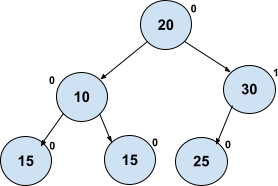
\includegraphics[height=100px]{./images/exam_2_avl_06_crop.png} \\\hline
\end{tabular}
\end{center}
\end{solution}

\noindent\textit{(c) After inserting 28 — rotation case, steps, final tree} \hfill (4 pts)

\begin{solution}

\begin{center}
\renewcommand{\arraystretch}{1.7}
\begin{tabular}{|p{1.8in}|p{1.8in}|p{1.8in}|}
  \hline 
  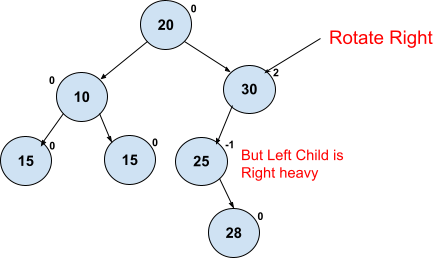
\includegraphics[height=100px]{./images/exam_2_avl_07_crop.png} & 
  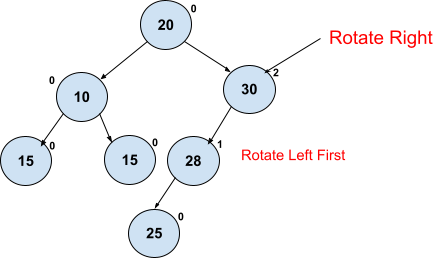
\includegraphics[height=100px]{./images/exam_2_avl_08_crop.png} & 
  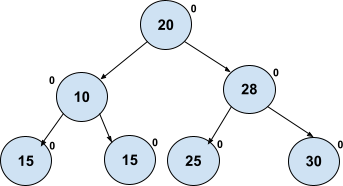
\includegraphics[height=100px]{./images/exam_2_avl_09_crop.png} \\\hline
\end{tabular}
\end{center}
\end{solution}


% ════════════════════════════════════════════════════════════════════════════
\newpage
\thispagestyle{empty}

\begin{center}
  {\large\bfseries Answer Sheet --- Exam 02, Page 2}\\[2pt]
  Name: \makebox[2.6in]{\hrulefill}
\end{center}

\noindent\rule{\linewidth}{0.6pt}

% ── SA3 ─────────────────────────────────────────────────────────────────────
\noindent\textbf{SA3 — Kruskal's Algorithm} \hfill \textit{/10}

\vspace{4pt}
\noindent\textit{(a) Trace table} \hfill (6 pts)

\begin{center}
\renewcommand{\arraystretch}{1.7}
\begin{tabular}{|c|c|c|c|p{2.5in}|}
  \hline
  \textbf{Step} & \textbf{Edge} & \textbf{Wt} & \textbf{Action} & \textbf{Components after}\\\hline
  1 & & & & \\\hline
  2 & & & & \\\hline
  3 & & & & \\\hline
  4 & & & & \\\hline
  5 & & & & \\\hline
  6 & & & & \\\hline
  7 & & & & \\\hline
\end{tabular}
\end{center}

\noindent\textit{(b) MST edges and total weight} \hfill (2 pts)
\answerlines{4}

\noindent\textit{(c) Why B--C is skipped (Union-Find)} \hfill (2 pts)
\answerlines{6}

\noindent\rule{\linewidth}{0.4pt}

\newpage
% ── SA4 ─────────────────────────────────────────────────────────────────────
\noindent\textbf{SA4 — Huffman Tree} \hfill \textit{/10}

\vspace{4pt}
\noindent\textit{(a) Min-heap merge trace} \hfill (3 pts)

\begin{center}
\renewcommand{\arraystretch}{1.7}
\begin{tabular}{|c|p{1.8in}|p{1.8in}|c|}
  \hline
  \textbf{Step} & \textbf{Left (weight)} & \textbf{Right (weight)} & \textbf{New weight}\\\hline
  1 & & & \\\hline
  2 & & & \\\hline
  3 & & & \\\hline
  4 & & & \\\hline
  5 & & & \\\hline
\end{tabular}
\end{center}

\noindent\textit{(b) Huffman tree sketch (0 = left edge, 1 = right edge)} \hfill (3 pts)

\vspace{144pt} % drawing space

\newpage
\noindent\textit{(c) Encoding table and bit totals} \hfill (4 pts)

\begin{center}
\renewcommand{\arraystretch}{1.5}
\begin{tabular}{|c|c|c|c|c|}
  \hline
  \textbf{Char} & \textbf{Freq} & \textbf{Code} & \textbf{Length} &
  \textbf{Bits (F$\times$L)}\\\hline
  A & 12 & & & \\\hline
  B &  7 & & & \\\hline
  C &  5 & & & \\\hline
  D &  4 & & & \\\hline
  E &  3 & & & \\\hline
  F &  2 & & & \\\hline
  \multicolumn{4}{|r|}{\textbf{Total Huffman bits:}}  & \\\hline
  \multicolumn{4}{|r|}{\textbf{Fixed 3-bit ($33\times3$):}} & 99 \\\hline
  \multicolumn{4}{|r|}{\textbf{Bits saved:}}  & \\\hline
\end{tabular}
\end{center}

\end{document}
